\documentclass{ximera}
%% You can put user macros here
%% However, you cannot make new environments

\listfiles

\graphicspath{{./}{firstExample/}{secondExample/}}

\usepackage{tikz}
\usepackage{tkz-euclide}
\usepackage{tikz-3dplot}
\usepackage{tikz-cd}
\usetikzlibrary{shapes.geometric}
\usetikzlibrary{arrows}
\usetkzobj{all}
\pgfplotsset{compat=1.13} % prevents compile error.

%\renewcommand{\vec}[1]{\mathbf{#1}}
\renewcommand{\vec}{\mathbf}
\newcommand{\RR}{\mathbb{R}}
\newcommand{\dfn}{\textit}
\newcommand{\dotp}{\cdot}
\newcommand{\id}{\text{id}}
\newcommand\norm[1]{\left\lVert#1\right\rVert}
 
\newtheorem{general}{Generalization}
\newtheorem{initprob}{Exploration Problem}

\tikzstyle geometryDiagrams=[ultra thick,color=blue!50!black]

%\DefineVerbatimEnvironment{octave}{Verbatim}{numbers=left,frame=lines,label=Octave,labelposition=topline}



\usepackage{mathtools}

\author{Anastasiia Holovchenko \and Anna Davis (project advisor)} \title{Applying the Central Limit Theorem} 
\begin{document}
\begin{abstract}
\end{abstract}
\maketitle


\section{Voluntary Consent} 
I have read the \href{https://ximera.osu.edu/statproj/CLTtoHT/consent/main}{Consent Form} and understand what is being requested of me.  I also understand that my participation is voluntary and that I am free to withdraw consent at any time, for any reason while accessing this platform.

 \begin{question} 
Are you 18 years of age or older? Type YES or NO in the space below.  
\begin{freeResponse}  
\end{freeResponse}  
\end{question}

\begin{question}  
Do you give us permission to use the data from your session in our study?  Type YES or NO in the space below. 
\begin{freeResponse}  
\end{freeResponse}  
\end{question}

\section{Problems}
To complete the following assignment, you need to be familiar with the Empirical Rule and the Central Limit Theorem.

{\color{red}You have an UNLIMITED number of tries for each question.  If you get the answer wrong, try again!}

\begin{problem}\label{pr:cheesecake}
A restaurant claims that their cheesecake dessert contains 400 calories, with a known population standard deviation of 25 calories. A food critic suspects that the dessert contains more calories than the restaurant claims and decides to take a random sample of 100 cheesecakes to test the restaurant's claim. The critic finds that the sample mean is 410 calories. Answer the questions below:

\begin{question} 
Identify the following:
\begin{enumerate}
    \item $\mu$ (presumed population mean) $= \answer{400}$
    \item $\sigma$ (population standard deviation) $= \answer{25}$
    \item $\bar{x}$ (sample mean) $=\answer{410}$
    \item $n$ (sample size) $= \answer{100}$
\end{enumerate}
\end{question}

\begin{question} Select the correct formula for calculating standard deviation for a sampling distribution.

\begin{multipleChoice}  
    \choice{$\sigma_{\bar{x}} = \sigma(n+1)/\sqrt{n}$}  
    \choice[correct]{$\sigma_{\bar{x}} =\sigma/\sqrt{n}$}  
    \choice{$\sigma_{\bar{x}}  = \sigma /\sqrt{n+1}$}  
    \choice{$\sigma_{\bar{x}} = \frac{b-a}{\sqrt{12}}$}  
\end{multipleChoice} 

\end{question}

\begin{question} Using the correct formula, determine the value of standard deviation for the sampling distribution:
$$\mbox{St. dev. for sampling distribution:}\quad\sigma_{\bar{x}}= \answer{2.5}$$
\end{question}

\begin{question} From the choices below, pick the graph that represents the sampling distribution, assuming that the mean is 400 calories. %[MAYBE MAKE A VIDEO HERE ON HOW TO MAKE THE GRAPH]

\begin{multipleChoice}
\choice{
      \begin{tikzpicture}
        \begin{axis}[
          domain=320:480,
          xmin=320, xmax=480,
          ymin=-0.01, ymax=0.03,
          width=3.5in,
          xtick={325,350, 375,400,425,450,475},
            xticklabels={$325$,$350$,$375$,$400$, $425$,$450$,$475$},
           % ytick style={draw=none},
            %yticklabels={},
            axis x line=center,
            axis y line=none,
          %axis lines =middle, xlabel={}, ylabel={},
          %every axis y label/.style={at=(current axis.above origin),anchor=south},
           every axis x label/.style={at=(current axis.right of origin),anchor=west},
          ]
      \addplot [very thick,  smooth] {(e^(-0.5*((x-400)/25)^2))/(((2*pi)^0.5)*25)};
      %    \node at (axis cs:320, 0.025 ) [anchor=west] {$A$};
          \end{axis}
        \end{tikzpicture}
}
\choice[correct]{
       \begin{tikzpicture}
        \begin{axis}[
          domain=390:410,
          xmin=390, xmax=410,
          ymin=-0.01, ymax=0.3,
          width=3.5in,
          xtick={392.5, 395, 397.5,400,402.5,405, 407.5},
            xticklabels={$392.5$,$395$,$397.5$,$400$, $402.5$,$405$,$407.5$},
           % ytick style={draw=none},
            %yticklabels={},
            axis x line=center,
            axis y line=none,
          %axis lines =middle, xlabel={}, ylabel={},
          %every axis y label/.style={at=(current axis.above origin),anchor=south},
           every axis x label/.style={at=(current axis.right of origin),anchor=west},
          ]
      \addplot [very thick,  smooth] {(e^(-0.5*((x-400)/2.5)^2))/(((2*pi)^0.5)*2.5)};
          %\node at (axis cs:395, 0.25 ) [anchor=west] {$B$};
          \end{axis}
        \end{tikzpicture}
        }
        \choice{
        \begin{tikzpicture}
        \begin{axis}[
          domain=400:420,
          xmin=400, xmax=420,
          ymin=-0.01, ymax=0.03,
          width=3.5in,
          xtick={402.5, 405, 407.5,410,412.5,415,417.5},
            xticklabels={$402.5$,$405$,$407.5$,$410$, $412.5$,$415$,$417.5$},
           % ytick style={draw=none},
            %yticklabels={},
            axis x line=center,
            axis y line=none,
          %axis lines =middle, xlabel={}, ylabel={},
          %every axis y label/.style={at=(current axis.above origin),anchor=south},
           every axis x label/.style={at=(current axis.right of origin),anchor=west},
          ]
      \addplot [very thick,  smooth] {(e^((-(x-410)^2)/(2*2.5^2)))/(2*pi*2.5^2)};
         % \node at (axis cs:405, 0.025 ) [anchor=west] {$C$};
          \end{axis}
        \end{tikzpicture}
        }
        \choice{
        \begin{tikzpicture}
        \begin{axis}[
          domain=330:490,
          xmin=330, xmax=490,
          ymin=-0.01, ymax=0.03,
          width=3.5in,
          xtick={335,360,385,410,435,460,485},
            xticklabels={$335$,$360$,$385$,$410$, $435$,$460$,$385$},
           % ytick style={draw=none},
            %yticklabels={},
            axis x line=center,
            axis y line=none,
          %axis lines =middle, xlabel={}, ylabel={},
          %every axis y label/.style={at=(current axis.above origin),anchor=south},
           every axis x label/.style={at=(current axis.right of origin),anchor=west},
          ]
      \addplot [very thick,  smooth] {(e^(-0.5*((x-410)/25)^2))/(((2*pi)^0.5)*25)};
         % \node at (axis cs:360, 0.025 ) [anchor=west] {$D$};
          \end{axis}
        \end{tikzpicture}
 }
\end{multipleChoice}
\end{question}

\begin{question}
    Refer to the (correct) graph you selected above.  Where does the sample mean $\bar{x}=410$ fall?

    \begin{multipleChoice}
\choice{In the center}
\choice{Less than one standard deviation to the right of the mean}
\choice{Approximately two standard deviations to the right of the mean}
\choice[correct]{Four standard deviations to the right of the mean}
\end{multipleChoice}
\end{question}

\begin{question}
If the restaurant is correct in saying that the average calorie count per cheesecake is 400, how likely is a sample of 100 cheesecakes to have an average calorie count of 410 or greater?
\begin{multipleChoice}
\choice{Likely}
\choice{Somewhat likely}
\choice{Unlikely}
\choice[correct]{Highly unlikely}
\end{multipleChoice}
\end{question}
\begin{question}
Based on your answer above, do you think the restaurant is being truthful about the average calorie count in their cheesecake?
\begin{multipleChoice}
\choice{Yes}
\choice[correct]{No}
\end{multipleChoice}
\end{question}

\end{problem}

\subsection{Discussion}  In Problem \ref{pr:cheesecake}, you determined that the probability of getting a sample of 100 cheesecakes with a mean calorie count of 410 is pretty much impossible if the restaurant is correct in claiming that the mean calorie count is 400.  This decision was based on the Empirical Rule which states that $99.7\%$ of normally distributed data are contained within three standard deviations of the mean.  Since our sample mean $\bar{x}=410$ is outside of the $99.7\%$ interval, we concluded that such a sample is impossible, given the population mean of 400.  This lead us to conclude that the population mean cannot be 400. 

\begin{problem}\label{pr:chips}
A potato chips company claims that, on average, their package contains 200 grams of potato chips. Based on many years of testing, it is known that the population standard deviation is 10 grams and the amounts are normally distributed. Suppose that the company headquarters suspects that the manufacturer is routinely under-filling the packs of chips to cut cost. The company headquarters sends an inspector to the plant to find out what’s going on. The inspector takes a random sample of 25 bags of chips and finds that the average mass is 198 grams. 

\begin{question} 
Identify the following:
\begin{enumerate}
    \item $\mu$ (presumed population mean) $= \answer{200}$
    \item $\sigma$ (population standard deviation) $= \answer{10}$
    \item $\bar{x}$ (sample mean) $=\answer{198}$
    \item $n$ (sample size) $= \answer{25}$
\end{enumerate}
\end{question}

\begin{question}
Determine the value of standard deviation for the sampling distribution:
$$\mbox{St. dev. for sampling distribution:}\quad\sigma_{\bar{x}}= \answer{2}$$
\end{question}

\begin{question}
Choose the correct graph for the sampling distribution, assuming that the mean mass for the population is 200g:
\begin{multipleChoice}
\choice[correct]{
      \begin{tikzpicture}
        \begin{axis}[
          domain=190:210,
          xmin=190, xmax=210,
          ymin=-0.01, ymax=0.3,
          width=3.5in,
          xtick={194,196, 198, 200, 202, 204, 206},
            xticklabels={$194$,$196$,$198$,$200$,$202$,$204$,$206$},
           % ytick style={draw=none},
            %yticklabels={},
            axis x line=center,
            axis y line=none,
          %axis lines =middle, xlabel={}, ylabel={},
          %every axis y label/.style={at=(current axis.above origin),anchor=south},
           every axis x label/.style={at=(current axis.right of origin),anchor=west},
          ]
      \addplot [very thick,  smooth] {(e^(-0.5*((x-200)/2)^2))/(((2*pi)^0.5)*2)};
      %    \node at (axis cs:320, 0.025 ) [anchor=west] {$A$};
          \end{axis}
        \end{tikzpicture}
}
\choice{
       \begin{tikzpicture}
        \begin{axis}[
          domain=190:206,
          xmin=190, xmax=206,
          ymin=-0.01, ymax=0.3,
          width=3.5in,
          xtick={192,194, 196, 198, 200, 202, 204},
            xticklabels={$192$,$194$,$196$,$198$,$200$,$202$,$204$},
           % ytick style={draw=none},
            %yticklabels={},
            axis x line=center,
            axis y line=none,
          %axis lines =middle, xlabel={}, ylabel={},
          %every axis y label/.style={at=(current axis.above origin),anchor=south},
           every axis x label/.style={at=(current axis.right of origin),anchor=west},
          ]
      \addplot [very thick,  smooth] {(e^(-0.5*((x-198)/2)^2))/(((2*pi)^0.5)*2)};
      %    \node at (axis cs:320, 0.025 ) [anchor=west] {$A$};
          \end{axis}
        \end{tikzpicture}
        }
\choice{
        \begin{tikzpicture}
        \begin{axis}[
          domain=160:240,
          xmin=160, xmax=240,
          ymin=-0.01, ymax=0.3,
          width=3.5in,
          xtick={170,180, 190, 200, 210, 220, 230},
            xticklabels={$170$,$180$,$190$,$200$,$210$,$220$,$230$},
           % ytick style={draw=none},
            %yticklabels={},
            axis x line=center,
            axis y line=none,
          %axis lines =middle, xlabel={}, ylabel={},
          %every axis y label/.style={at=(current axis.above origin),anchor=south},
           every axis x label/.style={at=(current axis.right of origin),anchor=west},
          ]
      \addplot [very thick,  smooth] {(e^(-0.5*((x-200)/10)^2))/(((2*pi)^0.5)*2)};
      %    \node at (axis cs:320, 0.025 ) [anchor=west] {$A$};
          \end{axis}
        \end{tikzpicture}
        }
\choice{
\begin{tikzpicture}
        \begin{axis}[
          domain=160:230,
          xmin=160, xmax=230,
          ymin=-0.01, ymax=0.3,
          width=3.5in,
          xtick={168, 178, 188, 198, 208, 218, 228},
            xticklabels={$168$,$178$,$188$,$198$,$208$,$218$,$228$},
           % ytick style={draw=none},
            %yticklabels={},
            axis x line=center,
            axis y line=none,
          %axis lines =middle, xlabel={}, ylabel={},
          %every axis y label/.style={at=(current axis.above origin),anchor=south},
           every axis x label/.style={at=(current axis.right of origin),anchor=west},
          ]
      \addplot [very thick,  smooth] {(e^(-0.5*((x-195)/10)^2))/(((2*pi)^0.5)*2)};
      %    \node at (axis cs:320, 0.025 ) [anchor=west] {$A$};
          \end{axis}
        \end{tikzpicture}
}
        
\end{multipleChoice}
\end{question}

\begin{question}
Assuming that the potato chips company does put 200g of potato chips in a bag, on average, what is the probability of obtaining a sample of 25 bags that, on average, contain 198g or less per bag?
\begin{multipleChoice}
\choice{approximately $68\%$}
\choice[correct]{approximately $16\%$}
\choice{approximately $99.7\%$}
\choice{approximately $3.4\%$}
\end{multipleChoice}
\begin{hint}
Use the Empirical rule.
\end{hint}
\end{question}

% \begin{question}
% Is the potato chips company telling the truth about having 200 grams of chips in a bag?
% \begin{multipleChoice}
% \choice{Yes}
% \choice[correct]{No}
% \end{multipleChoice}
% \end{question}

\end{problem}

\subsection{Discussion} Did the inspector in Problem \ref{pr:chips} find enough evidence to say that the manufacturer is under-filling the bags and the mean mass is less than 200 grams?  In the last question you had found that the probability of getting a sample of size 25 with an average amount of 198 grams or less is approximately $16\%$.  Should we consider this a ``likely" or an ``unlikely" probability?  Guidelines vary slightly from discipline to discipline but in general, we consider events that have less than five percent probability of occurring to be \emph{unlikely}.  If the probability of an event is greater than five percent, then we consider it to be reasonably likely.  With this in mind, we can say that it is reasonably likely that the bags in the inspector's sample of 25 would, on average, contain 198 grams or less. The inspector's findings do NOT contradict the manufacturer's claim that the mean amount is 200 grams.  At this point in time, we do NOT have enough evidence to conclude that the plant is under-filling the chip bags.

 % \begin{question}
 % How many standard deviations away from the mean is considered "highly unlikely"?
 % \begin{multipleChoice}
 % \choice{1 std}
 % \choice{2 std}
 % \choice[correct]{3 std}
 % \end{multipleChoice}
 % \end{question}

\begin{problem}\label{pr:bars}
Suppose a company manufactures snack bars. The company claims that the average mass of their granola bar is 130 grams and it is known that the population standard deviation is 6 grams. After a routine check a technician states that the machine might be broken and the average mass of granola bars is definitely greater than 130 grams. The company decides to test the technician's claim and collects a random sample of 36 granola bars. The average mass for the sample turns out to be 133 grams.

\begin{question}
Please identify the following:
 \begin{enumerate}
     \item $\mu$ (presumed population mean) $= \answer{130}$
     \item $\sigma$ (population standard deviation) $= \answer{6}$
     \item $\bar{x}$ (sample mean) $=\answer{133}$
     \item $n$ (sample size) $= \answer{36}$
\end{enumerate}
\end{question}

\begin{question}
Determine the value of standard deviation for the sampling distribution:
$$\mbox{St. dev. for sampling distribution:}\quad\sigma_{\bar{x}}= \answer{1}$$
\end{question}

\begin{question}
    Consider the sampling distribution curve.  Where is 133 grams located in relation to the presumed mean of 130 grams?
    \begin{multipleChoice}
 \choice{In the center}
 \choice{One standard deviation to the right}
 \choice{Two standard deviations to the right}
 \choice[correct]{Three standard deviations to the right}
 \end{multipleChoice}
\end{question}

% \begin{question}
% What is the acceptable range of the weight of the granola bar:
% If we were to take thousands of samples each containing 36 bars, approximately $68\%$ of the samples would lie in what range?
% \end{question}
% \begin{hint}
% Use the Empirical rule.
% \end{hint}
% \begin{multipleChoice}
% \choice[correct]{129 - 131 grams}
% \choice{124 - 136 grams}
% \choice{128 - 132 grams}
% \choice{127 - 133 grams}
% \end{multipleChoice}
% \end{question}


 \begin{question}
 Assuming that the equipment is functioning properly and the mean mass of bars is 130 grams, how likely is a sample mean of 133 grams or greater to occur for a sample of 36 bars?
 \begin{multipleChoice}
 \choice{Likely}
 \choice{Somewhat likely}
 \choice[correct]{Unlikely}
 \end{multipleChoice}
 \end{question}

 \begin{question}
     Does this sample provide enough evidence that the technician is correct in claiming that the machine is malfunctioning and making larger granola bars?
     \begin{multipleChoice}
 \choice{No}
  \choice[correct]{Yes}
 \end{multipleChoice}
 \end{question}

 \end{problem}


\begin{problem}\label{pr:farmerJoe}
Farmer Joe is looking to sell his farm along with the animals. Emily is interested in buying the farm. To make the offer sound more appealing, Farmer Joe states that his chickens lay 10 eggs per week on average (with a standard deviation of 2).  The national average is only 6 eggs per week. Emily wants to test Joe's claim and decides to see for herself how many eggs Joe's chickens will produce in 1 week. To do so, she selects a random sample of 100 chickens. We will discuss Emily's findings later.  For now, you should be able to answer the following two questions.

\begin{question}
Please identify the following:
 \begin{enumerate}
     \item $\mu$ (presumed population mean) $= \answer{10}$
     \item $\sigma$ (population standard deviation) $= \answer{2}$
     \item $n$ (sample size) $= \answer{100}$
\end{enumerate}
\end{question}

\begin{question}
Determine the value of standard deviation for the sampling distribution:
$$\mbox{St. dev. for sampling distribution:}\quad\sigma_{\bar{x}}= \answer{0.2}$$
\end{question}

% \begin{question} Pick the correct graph that represents the sampling distribution, assuming that the mean is 6 eggs/week. %[MAYBE MAKE A VIDEO HERE ON HOW TO MAKE THE GRAPH]

% \begin{multipleChoice}
% \choice[correct]{
%       \begin{tikzpicture}
%         \begin{axis}[
%           domain=5:7,
%           xmin=5, xmax=7,
%           ymin=-0.01, ymax=0.03,
%           width=3.5in,
%           xtick={5.4, 5.6, 5.8, 6, 6.2, 6.4, 6.6},
%             xticklabels={$5.4$,$5.6$,$5.8$,$6$,$6.2$,$6.4$,$6.6$},
%            % ytick style={draw=none},
%             %yticklabels={},
%             axis x line=center,
%             axis y line=none,
%           %axis lines =middle, xlabel={}, ylabel={},
%           %every axis y label/.style={at=(current axis.above origin),anchor=south},
%            every axis x label/.style={at=(current axis.right of origin),anchor=west},
%           ]
%       \addplot [very thick,  smooth] {(e^(-0.5*((x-6)/25)^2))/(((2*pi)^0.5)*0.2)};
%       %    \node at (axis cs:320, 0.025 ) [anchor=west] {$A$};
%           \end{axis}
%         \end{tikzpicture}
% }
% \choice{
%        \begin{tikzpicture}
%         \begin{axis}[
%           domain=-2:14,
%           xmin=-2, xmax=14,
%           ymin=-0.01, ymax=1,
%           width=3.5in,
%           xtick={0, 2, 4, 6, 8, 10, 12},
%             xticklabels={$0$, $2$, $4$, $6$, $8$, $10$, $12$},
%            % ytick style={draw=none},
%             %yticklabels={},
%             axis x line=center,
%             axis y line=none,
%           %axis lines =middle, xlabel={}, ylabel={},
%           %every axis y label/.style={at=(current axis.above origin),anchor=south},
%            every axis x label/.style={at=(current axis.right of origin),anchor=west},
%           ]
%       \addplot [very thick,  smooth] {(e^(-0.5*((x-6)/0.)^2))/(((2*pi)^0.5)*0.2)};
%           %\node at (axis cs:395, 0.25 ) [anchor=west] {$B$};
%           \end{axis}
%         \end{tikzpicture}
%         }
%         \choice{
%         \begin{tikzpicture}
%         \begin{axis}[
%           domain=8:11,
%           xmin=8, xmax=11,
%           ymin=-0.01, ymax=0.03,
%           width=3.5in,
%           xtick={8.9, 9.1, 9.3, 9.5, 9.7, 9.9, 10.1},
%             xticklabels={$8.9$, $9.1$, $9.3$, $9.5$, $9.7$, $9.9$, $10.1$},
%            % ytick style={draw=none},
%             %yticklabels={},
%             axis x line=center,
%             axis y line=none,
%           %axis lines =middle, xlabel={}, ylabel={},
%           %every axis y label/.style={at=(current axis.above origin),anchor=south},
%            every axis x label/.style={at=(current axis.right of origin),anchor=west},
%           ]
%       \addplot [very thick,  smooth] {(e^((-(x-9.5)^2)/(2*2.5^2)))/(2*pi*2.5^0.2)};
%          % \node at (axis cs:405, 0.025 ) [anchor=west] {$C$};
%           \end{axis}
%         \end{tikzpicture}
%         }
%         \choice{
%         \begin{tikzpicture}
%         \begin{axis}[
%           domain=3:16,
%           xmin=3, xmax=16,
%           ymin=-0.01, ymax=0.03,
%           width=3.5in,
%           xtick={3.5, 5.5, 7.5, 9.5, 11.5, 13.5, 15.5},
%             xticklabels={$335$,$360$,$385$,$410$, $435$,$460$,$385$},
%            % ytick style={draw=none},
%             %yticklabels={},
%             axis x line=center,
%             axis y line=none,
%           %axis lines =middle, xlabel={}, ylabel={},
%           %every axis y label/.style={at=(current axis.above origin),anchor=south},
%            every axis x label/.style={at=(current axis.right of origin),anchor=west},
%           ]
%       \addplot [very thick,  smooth] {(e^(-0.5*((x-9.5)/25)^2))/(((2*pi)^0.5)*2)};
%          % \node at (axis cs:360, 0.025 ) [anchor=west] {$D$};
%           \end{axis}
%         \end{tikzpicture}
%  }
% \end{multipleChoice}
% \end{question}
    
% \end{question}

Now we turn to Emily's findings.

\begin{question}Suppose Emily's sample mean is 9.9 eggs/week.  Does this constitute enough evidence that Farmer Joe is lying?
\begin{multipleChoice}
    \choice{Yes}
    \choice[correct]{No}
\end{multipleChoice}
\end{question}

\begin{question}Suppose Emily's sample mean is 9.8 eggs/week.  Does this constitute enough evidence that Farmer Joe is lying?
\begin{multipleChoice}
    \choice{Yes}
    \choice[correct]{No}
\end{multipleChoice}
\end{question}

\begin{question}Suppose Emily's sample mean is 9.6 eggs/week.  Does this constitute enough evidence that Farmer Joe is lying?
\begin{multipleChoice}
    \choice[correct]{Yes}
    \choice{No}
\end{multipleChoice}
\end{question}

\end{problem}

\section{How to Get Your Certificate}
Thank you for attempting the problems.  You will need to take a screenshot of your certificate and submit it to your instructor.  Your certificate will look like this:

\begin{image}
         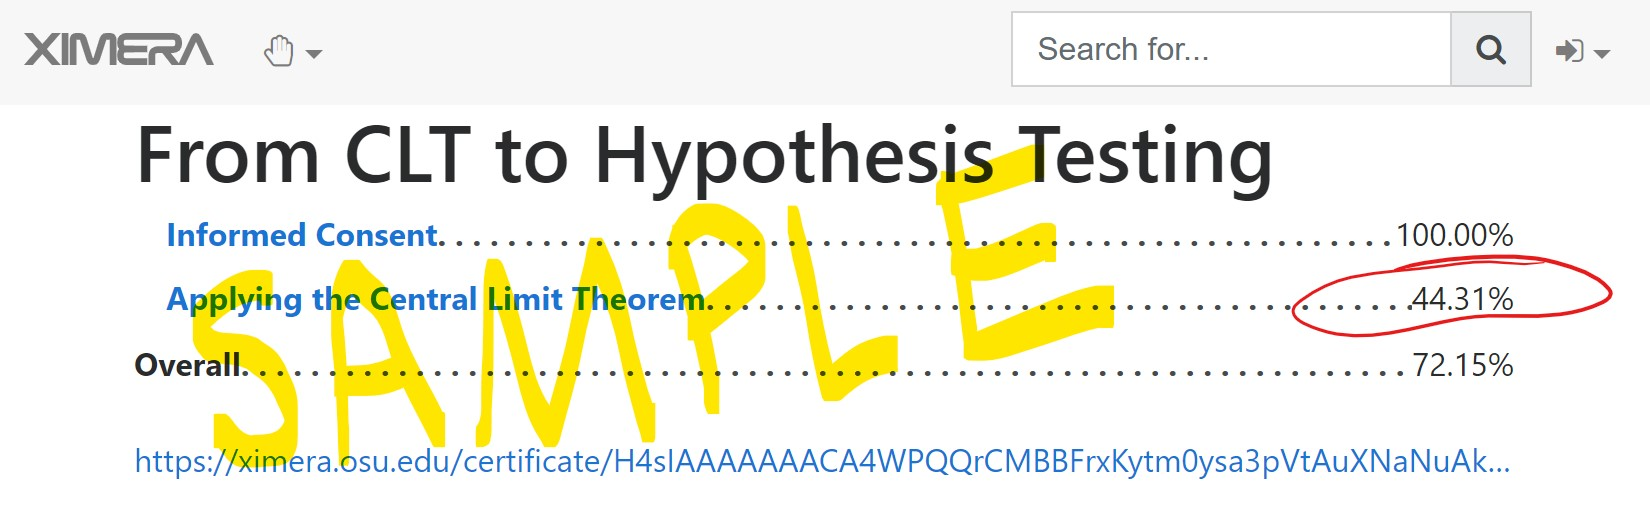
\includegraphics[height=1.5in]{certificate.jpg}
\end{image}

To obtain your certificate, return to the \href{https://ximera.osu.edu/statproj/CLTtoHT}{Landing Page}, click on the Certificate button, then take a screenshot of your certificate.  Follow your instructor's directions for how to submit your certificate for credit.

\begin{image}
         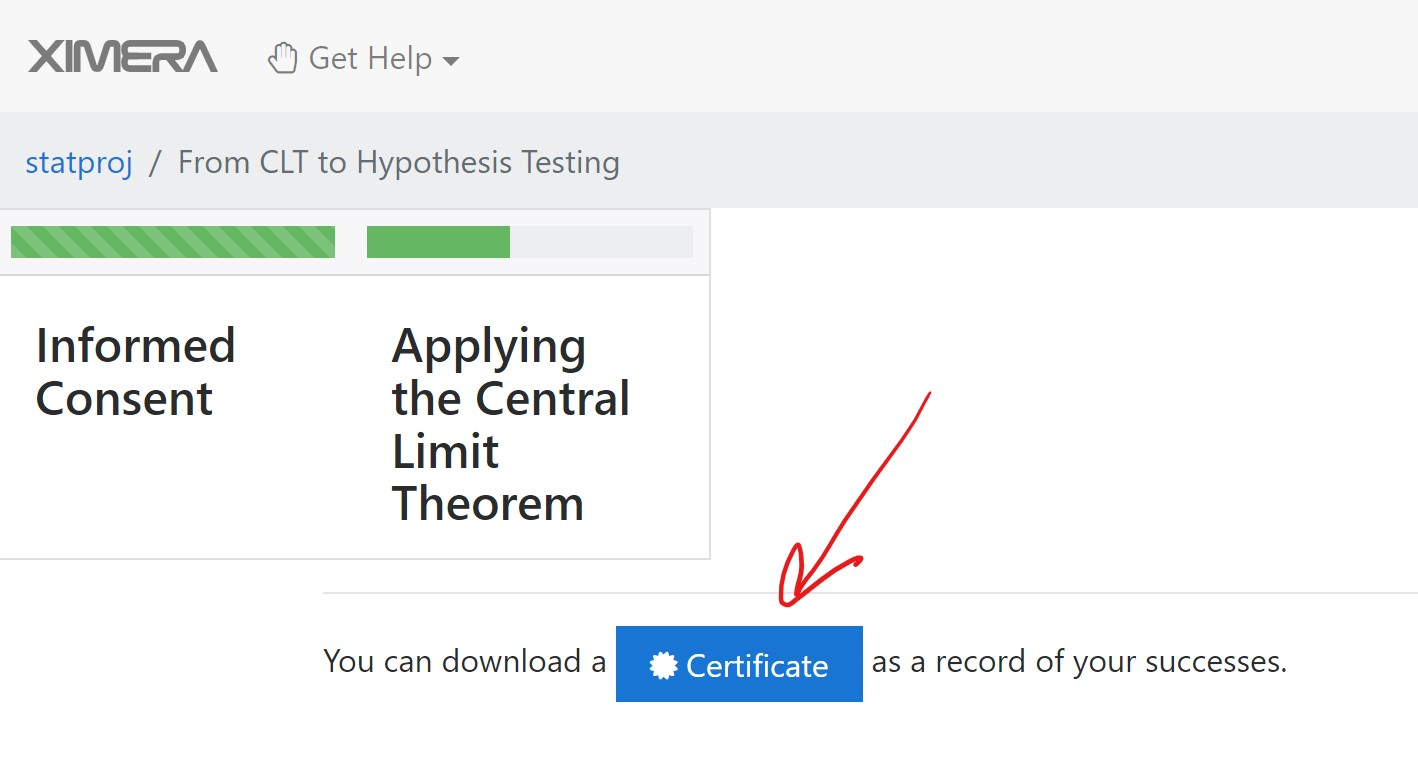
\includegraphics[height=2in]{certificate2.jpg}
\end{image}

For help with technical difficulties, please email Anna Davis at davisa@ohiodominican.edu.

\end{document} 